\documentclass[12pt,letterpaper]{article}

% packages
\usepackage[utf8]{inputenc}
\usepackage[margin=1in]{geometry}
\usepackage{setspace}
\usepackage[T1]{fontenc}
\usepackage{amsmath}
\usepackage{times}
\usepackage{graphicx}
\usepackage{hyperref}
\usepackage[font=footnotesize]{caption}
\usepackage{relsize}
\usepackage{environ}
\usepackage[skip=0.5cm]{parskip}
\usepackage[sorting=none]{biblatex}
\usepackage{tikz}
\usepackage{pgfplots}
\usepackage{paralist}
\usepackage{amssymb}
\usepackage{listings}
\usepackage{color}
\usepackage{titling}
\usepackage{blindtext}
\usepackage{titlesec}
\usepackage{subcaption}
\usepackage{multicol}
\usepackage{abstract}

% --- stuff from google ---
\edef\origparind{\the\parindent}
\usetikzlibrary{positioning}
\pgfplotsset{compat=1.16}
\parindent=\origparind\relax
\DeclareCaptionType{equ}[][]
\emergencystretch=2em

\makeatletter
\def\maketag@@@#1{\hbox{\m@th\normalfont\normalsize#1}}
\makeatother

% make text lines be further away from each other
%\setstretch{1.4}
\linespread{1.4}

% env for equations and mathematical expressions
\NewEnviron{EQUATIONS}{%
  \scalebox{1.25}{$\BODY$}
}

% set size and (something else?) for the section and subsection headers (I think)
\titleformat*{\section}{\large\bfseries}
\titleformat*{\subsection}{\normalsize\bfseries}

% make abstract header larger
\renewcommand{\abstractnamefont}{\normalfont\large\bfseries}
% --- stuff from google END ---

\addbibresource{bibliography.bib}

\title{\textbf{Speeding up Genotyping through GPU Acceleration}}
\date{15th of May 2023}
\author{\Large{Master's Thesis}\\\\Jørgen Wictor Henriksen}

\begin{document}

% title
\maketitle
\newpage

% abstract
\begin{abstract}
In the last few decades, high-throughput sequencing has steadily become more cost effective and accessible.
%When sequencing a human genome today, it is not uncommon to produce hundreds of millions of short snippets of the genetic sequence.
%These snippets are produced without knowledge of where they originate from in the original genome sequence or which bases in the snippet may be erroneous.
With the potential for millions of genomes being sequenced in the coming years, tools for analyzing the large amounts of genetic sequence data produced will become increasingly important.
Genotyping - the process of determining the genetic sequence variants present in the chromosomes of a genome - is a core application for such genetic sequence data.
Work in alignment-free genotyping, a new method that forgoes aligning each sequenced snippet to a reference genome sequence, have recently showed that statistical models on analysis of \textit{k}mers can yield competitive accuracies while being significantly faster compared to more traditional alignment-based methods.
A recently published genotyping tool, KAGE, showed that an alignment-free genotyper implemented in Python could yield competitive accuracies while being more than 10 times faster than any other known method.
This thesis explores how parts of KAGE, that is implemented in Python and deal with large matrix- and array-operations, can be GPU accelerated using a number of different methods with different advantages and shortcomings. 
We then finally present GKAGE, a GPU accelerated version of KAGE. 
GKAGE achieves up to 10 times speedup compared to KAGE and is able to genotype a human individual in only a few minutes on consumer grade hardware - significantly faster than any other known genotyping tool today.
We believe that the results achieved indicate that existing bioinformatics tools can benefit greatly from GPU acceleration.
\end{abstract}

\newpage

% table of contents
\tableofcontents
\newpage

% sections
\section{Introduction} \label{introduction}

A central problem in biology is to effectively uncover and characterize genetic sequence variations in humans.
By understanding where and how the human genome varies from individual to individual, we can vastly improve our understanding of how an individual's genetic makeup affects its observable traits - its phenotype.
To realize this goal, it is inescapable that we need fast and reliable methods for genotyping - characterizing an individual's genetic makeup - in order to gather data to further explore links between genotypes and phenotypes.

As the price of high-throughput sequencing has steadily become cheaper over the last few decades \cite{nhgri_sequencing_cost}, whole genome sequencing of human genomes has become more accessible than ever before.
Today, we can relatively cheaply sequence a whole human genome and expect to receive millions of short polynucleotide reads (often of length $\sim$ 150) \cite{illumina_read_length}.
From just such reads, where we neither know where the read originates from in the sequence's genome or where it may be erroneous, we want to perform the difficult task of accurately genotyping the individual, and to perform this analysis as quickly as possible.

The traditional and more established methods for genotyping a human individual have involved aligning all sequenced reads to a reference genome to examine where the reads differ from the reference, noting the genotypes supported.
Such \textit{alignment-based} methods are computationally expensive and time consuming, with established genotypers such as GATK \cite{gatk} needing tens of gigabytes of memory and several hours to run \cite{kage}.
In recent years, new \textit{alignment-free} strategies for genotyping human individuals have emerged.
Because of work such as the 1000 Genomes Project \cite{1000_genomes_project}, we today have access to vast amounts of knowledge about human genetic variation and genotype information.
Alignment-free genotyping methods leverage such knowledge to skip the taxing alignment step altogether in favour of genotyping individuals directly based on analysis of \textit{k}mers - short substrings of the read sequences - and previous knowledge of known genetic variation \cite{kage,malva}.
Recently, a new genotyping tool, KAGE, showed that by deploying an alignment-free method, it is possible to yield competitive genotype prediction accuracies while being an order of magnitude faster than any other known genotyper \cite{kage}.

In recent years, with the introduction of the \textit{general purpose graphical processing unit} (GPGPU), the \textit{graphical processing unit} (GPU) has become increasingly popular for solving problems that require heavy amounts of compute, with many such problems existing in the space of scientific computing.
Common for all traditional genotyping tools is that they are implemented to run on the \textit{central processing unit} (CPU).
This likely stems from the fact that memory usage commonly reaches tens, and sometimes hundreds of gigabytes when running these tools \cite{kage}, and that not all problems are fit to run on the GPU architecture.
However, the currently fastest known genotyping tool, KAGE, requires significantly less memory compared to its competitors.
Additionally, KAGE is implemented in Python, and performs a significant amount of large array operations - a type of operation well suited for the GPU architecture - using the Python library NumPy \cite{numpy}.
Because of this, KAGE seemingly stood to benefit from GPU acceleration.

In this thesis, we will explore whether we can speed up (alignment-free) genotyping in any significant way by utilizing the GPU.
We will start with KAGE as a base genotyper, and explore possible avenues for implementing GPU acceleration in KAGE to assess whether it results in significant speedup.
Since KAGE is implemented in Python and consists of several steps that can in effect be considered independent, several possible avenues for GPU acceleration are possible.
We will explore several of them to assess what options developers may have to GPU accelerate existing work in Python, and evaluate the advantages and drawbacks of each.



\newpage
\section{Background}
\subsubsection{DNA, Chromosomes and Genomes} \label{background:biology:dna_chromosomes_and_genomes}
\textit{Deoxyribonucleic acid} (DNA) is a type of molecule that carries the genetic instructions for the development, function, and reproduction of all known living organisms.
The molecule is composed of two connected strands that wind around each other into a double helix shape.
Each strand is made up of a sugar and phosphate backbone, with each sugar carrying one out of four bases, often referred to as \textit{nucleotides}. 
The four DNA nucleotides are: \textit{cytosine}, \textit{guanine}, \textit{adenine} and \textit{thymine}, and they are typically referred to by their abbreviations C, G, A and T respectively.
Furthermore, chemical bonds form between complementary pairs of nucleotides: AT/TA and CG/GC, meaning that A and T, and C and G are complementary. 
The two strands are connected by these bonds formed between these nucleotides.
Since the sequence of nucleotides in one strand is complementary to the other, the two strands do in fact encode the same genetic information.
In other words, by having one strand, the other can be determined by reversing the strand you have and then exchanging each nucleotide by its complement.

DNA is organized into structures called \textit{chromosomes}. 
Humans have 46 chromosomes made up by two sets of 23 chromosomes where each chromosome occurs twice. One is inherited from the male parent and the other is inherited from the female parent.

The \textit{genome} of an organism usually refers to the entirety of an organism's genetic information. 

\begin{figure}[ht!]
\begin{center}
\scalebox{1}{
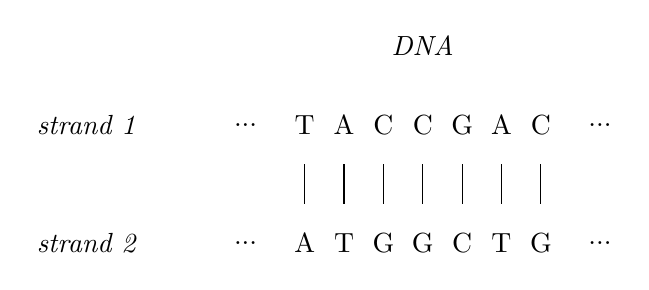
\begin{tikzpicture}
  % texts
  \node at(2.25,2.5)(title){\textit{DNA}};
  \node at(-2,0)(title){\textit{strand 2}};
  \node at(-2,1.5)(title){\textit{strand 1}};
  % lower nodes
  \node at(0,0)(n1){...};
  \node at(.75,0)(n2){A};
  \node at(1.25,0)(n3){T};
  \node at(1.75, 0)(n4){G};
  \node at(2.25,0)(n5){G};
  \node at(2.75,0)(n5){C};
  \node at(3.25,0)(n5){T};
  \node at(3.75,0)(n5){G};
  \node at(4.5,0)(n5){...};
  % upper nodes
  \node at(0,1.5)(n1){...};
  \node at(.75,1.5)(n2){T};
  \node at(1.25,1.5)(n3){A};
  \node at(1.75,1.5)(n4){C};
  \node at(2.25,1.5)(n5){C};
  \node at(2.75,1.5)(n5){G};
  \node at(3.25,1.5)(n5){A};
  \node at(3.75,1.5)(n5){C};
  \node at(4.5,1.5)(n5){...};
  % base pair bonds 
  \draw (.75,.5) -- (.75,1);
  \draw (1.25,.5) -- (1.25,1);
  \draw (1.75,.5) -- (1.75,1);
  \draw (2.25,.5) -- (2.25,1);
  \draw (2.75,.5) -- (2.75,1);
  \draw (3.25,.5) -- (3.25,1);
  \draw (3.75,.5) -- (3.75,1);
\end{tikzpicture}
}
\caption{A conceptual representation of a DNA molecule made up of two strands. The strands are composed of nucleotides forming base pairs where A (adenine) and T (thymine), and C (cytosine) and G (guanine) are complements of each other.}
\label{background:biology:dna_and_chromosomes:figures:dna_strands}
\end{center}
\end{figure}

Studying organisms' DNA is important for a variety of reasons.
It is particularly important to understand genetic diseases and how to best treat them.

...

\subsection{Variants and Variant Calling} \label{background:variants_and_variant_calling}
When examining the genome of several individuals within the same species, one will find locations along the genome where the nucleotides differ for the different individuals.
These distinct nucleotide manifestations are commonly referred to as \textit{variants}.
The term \textit{variant calling} is used to refer to the process of determining which variants an individual has.
In other words, given a reference genome sequence, where and how does the genome sequence of the individual of interest differ from the reference sequence.
This process can abstractly be described in three steps: 
1) sequence the genome of interest to get DNA reads (described in section \ref{background:high_throughput_dna_sequencing}), 
2) align the reads to the reference genome by finding where along the reference genome sequence each read fits best, usually using a heuristic determining which location the read originates from, and 
3) examine the alignments and note where and how the reference and the individual's sequences differ to determine the variants present in the individual's genome \cite{variant_calling}.

A common way to represent genome sequence variations is to encode them according to the \textit{Variant Call Format} (VCF) file format.
The VCF file format encodes a single variant per line, and each line contains a number of columns where each column encodes a particular piece of information about the associated variant, such as \cite{vcf}:
\begin{compactenum}
  \item
    CHROM: an identifier for the reference sequence used, \textit{i}.\textit{e}. the sequence against which the sequenced reads varies.
  \item
    POS: the position along the reference sequence where it varies against the sequenced reads.
  \item
    ID: an identifier for the variantion.
  \item
    REF: the reference base (or bases) found at the POS position in the reference sequence.
  \item
    ALT: a list of the alternative base (or bases) found at this POS position.
\end{compactenum}
While more columns are usually present, this encapsulated the necessary knowledge about variants and their representation needed for this thesis.

\definecolor{variantcolor}{RGB}{235,235,235}

\begin{figure}[H]
\begin{center}
\scalebox{1}{
\begin{tikzpicture}
  % texts
  \node at(2.75,2)(title){\small{\textit{observed variant}}};
  \node at(-3.525,-1)(title){\textit{reference sequence index}};
  \node at(-3,0)(title){\textit{reference sequence}};
  \node at(-2.715,1)(title){\textit{sequenced read}};
  % color boxes
  \node at(2.75,0.5)[rounded corners,minimum width=0.5cm,minimum height=1.65cm, fill=variantcolor](variant){};
  % indices
  \node at(0,-1)(n1){$...$};
  \node at(.75,-1)(n2){\small{3}};
  \node at(1.25,-1)(n3){\small{4}};
  \node at(1.75,-1)(n4){\small{5}};
  \node at(2.25,-1)(n5){\small{6}};
  \node at(2.75,-1)(n5){\small{7}};
  \node at(3.25,-1)(n5){\small{8}};
  \node at(3.75,-1)(n5){\small{9}};
  \node at(4.5,-1)(n5){$...$};
  % lower nodes
  \node at(0,0)(n1){$...$};
  \node at(.75,0)(n2){T};
  \node at(1.25,0)(n3){A};
  \node at(1.75,0)(n4){C};
  \node at(2.25,0)(n5){C};
  \node at(2.75,0)(n5){T};
  \node at(3.25,0)(n5){A};
  \node at(3.75,0)(n5){C};
  \node at(4.5,0)(n5){$...$};
  % upper nodes
  \node at(.75,1)(n2){T};
  \node at(1.25,1)(n3){A};
  \node at(1.75,1)(n4){C};
  \node at(2.25,1)(n5){C};
  \node at(2.75,1)(n5){G};
  \node at(3.25,1)(n5){A};
  \node at(3.75,1)(n5){C};
  % down arrow
  \draw [-stealth](0,-1.75) -- (0,-2.5);
  % POS 
  \node at(-1,-3.25)(vcf_pos){\small{POS}};
  \node at(0,-3.25)(vcf_pos){\small{:}};
  \node at(0.55,-3.25)(vcf_pos){\small{7}};
  % REF
  \node at(-1,-3.75)(vcf_ref){\small{REF}};
  \node at(0,-3.75)(vcf_ref){\small{:}};
  \node at(0.55,-3.75)(vcf_ref){\small{T}};
  % ALT
  \node at(-1,-4.25)(vcf_alt){\small{ALT}};
  \node at(0,-4.25)(vcf_alt){\small{:}};
  \node at(0.55,-4.25)(vcf_alt){\small{G}};
\end{tikzpicture}
}
\caption{An illustration of how a sequenced read can be aligned to a reference sequence and the variant present in the sequenced read is determined and encoded in (a simplified) VCF format, where several of the common columns are omitted.}
\label{background:variant_and_variant_calling:figures:variants}
\end{center}
\end{figure}


\subsubsection{Genotype and Genotyping} \label{background:biology:genotype_and_genotyping}
The term \textit{genotype} refers to the set of variants an individual carries at a particular location along the genome sequence of all of its chromosomes \cite{nhgri_genotype}.
For humans, who have two of each chromosome, a genotype would refer to two variants, one in each of the two chromosomes.
\textit{Genotyping} an individual refers to the process of determining which genotypes an individual carries. 
In most genotyping software tools today, genotypes are given in a format that specifies whether a particular variant is present in none, one or both of a human's chromosomes.
For instance, given a reference genome sequence where a variant site is known to could manifest an A at a particular allele where the reference sequence contains a C, a human individual's genotype for this variant could either be referred to as $0/0$, meaning that the variant is present in neither of the chromosomes, $0/1$, meaning that the variant is present in one of the chromosomes, or $1/1$, meaning that the variant is present in both chromosomes.

\definecolor{variantcolor}{RGB}{235,235,235}

\begin{figure}[ht!]
\begin{center}
\scalebox{0.85}{
\begin{tikzpicture}
  % Variants
  \node at(2.25,2)(title){\textit{Variants}};
  \node at(2.25,0)[rounded corners,minimum width=0.5cm,minimum height=2.75cm, fill=variantcolor](variant){};
  % Sequence (left)
  \node at(0.75,0)(n2){\large A};
  \node at(1.25,0)(n3){\large T};
  \node at(1.75,0)(n4){\large G};
  \node at(2.25,1)(n5){\large C};
  \node at(2.25,0)(n5){\large G};
  \node at(2.25,-1)(n5){\large A};
  \node at(2.75,0)(n5){\large C};
  \node at(3.25,0)(n5){\large T};
  % Arrow
  \draw [-stealth](4,0) -- (5,0);
  % Genotype
  \node at(7.5,2.5)(title){\textit{Genotype}};
  \node at(9,0.25)[rectangle,rounded corners,draw,minimum width=7cm,minimum height=3.25cm](genotype){};
  % Alleles 
  \node at(7.5,1.5)(title){\textit{Alleles}};
  % Chromosomes
  \node at(10.5,0.5)(title){$Chromosome_1$};
  \node at(10.5,-0.5)(title){$Chromosome_2$};
  \node at(7.5,-.015)[rounded corners,minimum width=0.5cm,minimum height=1.75cm, fill=variantcolor](variant){};
  % Chromosome 1 sequence
  \node at(6,0.5)(n2){\large A};
  \node at(6.5,0.5)(n3){\large T};
  \node at(7,0.5)(n4){\large G};
  \node at(7.5,0.5)(n5){\large A};
  \node at(8,0.5)(n5){\large C};
  \node at(8.5,0.5)(n5){\large T};
  % Chromosome 2 sequence
  \node at(6,-0.5)(n2){\large A};
  \node at(6.5,-0.5)(n3){\large T};
  \node at(7,-0.5)(n4){\large G};
  \node at(7.5,-0.5)(n5){\large G};
  \node at(8,-0.5)(n5){\large C};
  \node at(8.5,-0.5)(n5){\large T};
  % Reference and the individual's chromosomes
  \node at(2.25,-2.5)(ref){\textit{Reference sequence}};
  \node at(9,-2.5)(ind){\textit{Individual's chromosome sequences}};
\end{tikzpicture}
}
\caption{In humans, where there are two chromosomes, a genotype constitutes as a set of two alleles, one in each chromosome at the variant location. Along the reference sequence on the left, several possible variants may be known to occur at a specific location. After examining the sequence of an individual, we try to determine the individual's genotype by scoring which variants are present in each chromosome at the location of interest.}
\label{figure:variant_and_genotype}
\end{center}
\end{figure}

The most established way to genotype an individual today is to align DNA reads to a reference genome sequence and then examine how the reads differ from the reference sequence to determine which variants are present, and which genotypes are most probable at the different locations \cite{gatk}.
However, given how many reads one have come to expect from high-throughput sequencing today [\ref{background:biology:high_throughput_dna_sequencing}] and how time consuming it is to align reads to a $3*10^9$ long reference sequence, although accurate, this strategy is very time consuming.
A new prominent strategy has emerged in recent years that helps to alleviate the time consumption aspect of genotyping.
Statistics based methods where the variant calling step is skipped altogether, and small parts of the DNA reads called \textit{k}mers are analyzed to then use bayesian models determine which genotypes are most probable given previous knowledge accumulated over years of research \cite{kage,malva,1000_genomes_project}.
One such baysian genotyper, KAGE, have recently showed that it can genotype a human individual more than 10 times faster than any other known genotyper tool, while still providing competitive accuracy scores \cite{kage}.

\subsubsection{High-Throughput DNA Sequencing} \label{background:biology:high_throughput_dna_sequencing}
\textit{High-throughput sequencing} (HTS), also known as \textit{next-generation sequencing} (NGS), refers to an assortment of recently developed technologies that parallelize the sequencing of DNA fragments to provide unprecedented amounts of genomic sequence data in short amounts of time.
While several such technologies with varying details exist today, they commonly follow a general paradigm. 
%This paradigm consists of performing a template preparation, clonal amplification where they clone pieces of DNA in order to sequence the clones in parallel, and finally cyclical rounds of massively parallel sequencing \cite{hts}.
This paradigm consists of performing a template preparation, clonal amplification where pieces of DNA are cloned in order to sequence the clones in parallel, and finally, cyclical rounds of massively parallel sequencing \cite{hts}.
The resulting DNA sequences produced by HTS technologies are usually referred to simply as (DNA) \textit{reads}.
Such reads are commonly stored as plain text in FASTA or FASTQ files, which can later be used for different kinds of analysis such as genotyping.
Depending on which HTS technology is used, one can expect read lengths ranging from as low as 150 bases using \textit{Illumina} technologies, referred to as \textit{short reads} \cite{illumina_read_length}, all the way up to 15-20 thousand bases using \textit{Pacific Biosciences} (PacBio) technologies, referred to as \textit{long reads} \cite{hts2}.
There are three important factors to consider when determining which HTS technology to use for a given purpose: 1) the read lengths produced, 2) the average probability for each base being erroneous, usually referred to as the error rate, and 3) the cost of sequencing given the technology, which can potentially limit how much data one may be able to produce.

\begin{figure}[H]
\begin{center}
\small{example.fa}
\end{center}
\begin{lstlisting}[style=vcf]
>read 0
ACGTATGCGGCGGGGCGCGATTATTCGTTGCGTATGC
>read 1
ACACGTCGTGCGTAGCGTGTCAGTCACAGTAAACAAA
>read 2
CGTTGCCATCAACGGCTGTGCACGATTGGGGGCGCGC
...
\end{lstlisting}
\caption{
  An illustration of how sequenced DNA reads are stored as plain text in a FASTA (.fa) file.
  Before each read, a header file beginning with the character ">" may provide information about the read.
}
\label{background:biology:high_throughput_dna_sequencing:figures:fasta}
\end{figure}

When performing DNA sequencing, we have no knowledge of where a read originates from in the original genome.
This issue, in addition to the fact that some bases are erroneously sequenced, introduces uncertainties when trying to predict features about an individual's genome based on the sequenced reads.
Many techniques rely on \textit{aligning} (or \textit{mapping}) sequenced reads to a reference genome sequence in order to better predict where in the genome the read originates from.
To gain better confidence and local support along these alignments, it is common to sequence an individual's genome at higher coverages, so that aligned reads may overlap and correspondance can be asserted.
The term sequencing \textit{coverage} is used as an indication of how many times each nucleotide in a genome has been sequenced on average.
E.g. 15x coverage means that every nucleotide in the genome has been sequenced, on average, 15 times.

\subsection{Biology} \label{background:biology}

\subsubsection{DNA, Chromosomes and Genomes} \label{background:biology:dna_chromosomes_and_genomes}
\textit{Deoxyribonucleic acid} (DNA) is a type of molecule that carries the genetic instructions for the development, function, and reproduction of all known living organisms.
The molecule is composed of two connected strands that wind around each other into a double helix shape.
Each strand is made up of a sugar and phosphate backbone, with each sugar carrying one out of four bases, often referred to as \textit{nucleotides}. 
The four DNA nucleotides are: \textit{cytosine}, \textit{guanine}, \textit{adenine} and \textit{thymine}, and they are typically referred to by their abbreviations C, G, A and T respectively.
Furthermore, chemical bonds form between complementary pairs of nucleotides: AT/TA and CG/GC, meaning that A and T, and C and G are complementary. 
The two strands are connected by these bonds formed between these nucleotides.
Since the sequence of nucleotides in one strand is complementary to the other, the two strands do in fact encode the same genetic information.
In other words, by having one strand, the other can be determined by reversing the strand you have and then exchanging each nucleotide by its complement.

DNA is organized into structures called \textit{chromosomes}. 
Humans have 46 chromosomes made up by two sets of 23 chromosomes where each chromosome occurs twice. One is inherited from the male parent and the other is inherited from the female parent.

The \textit{genome} of an organism usually refers to the entirety of an organism's genetic information. 

\begin{figure}[ht!]
\begin{center}
\scalebox{1}{
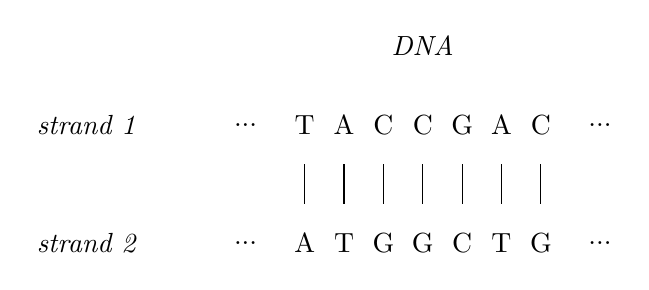
\begin{tikzpicture}
  % texts
  \node at(2.25,2.5)(title){\textit{DNA}};
  \node at(-2,0)(title){\textit{strand 2}};
  \node at(-2,1.5)(title){\textit{strand 1}};
  % lower nodes
  \node at(0,0)(n1){...};
  \node at(.75,0)(n2){A};
  \node at(1.25,0)(n3){T};
  \node at(1.75, 0)(n4){G};
  \node at(2.25,0)(n5){G};
  \node at(2.75,0)(n5){C};
  \node at(3.25,0)(n5){T};
  \node at(3.75,0)(n5){G};
  \node at(4.5,0)(n5){...};
  % upper nodes
  \node at(0,1.5)(n1){...};
  \node at(.75,1.5)(n2){T};
  \node at(1.25,1.5)(n3){A};
  \node at(1.75,1.5)(n4){C};
  \node at(2.25,1.5)(n5){C};
  \node at(2.75,1.5)(n5){G};
  \node at(3.25,1.5)(n5){A};
  \node at(3.75,1.5)(n5){C};
  \node at(4.5,1.5)(n5){...};
  % base pair bonds 
  \draw (.75,.5) -- (.75,1);
  \draw (1.25,.5) -- (1.25,1);
  \draw (1.75,.5) -- (1.75,1);
  \draw (2.25,.5) -- (2.25,1);
  \draw (2.75,.5) -- (2.75,1);
  \draw (3.25,.5) -- (3.25,1);
  \draw (3.75,.5) -- (3.75,1);
\end{tikzpicture}
}
\caption{A conceptual representation of a DNA molecule made up of two strands. The strands are composed of nucleotides forming base pairs where A (adenine) and T (thymine), and C (cytosine) and G (guanine) are complements of each other.}
\label{background:biology:dna_and_chromosomes:figures:dna_strands}
\end{center}
\end{figure}

Studying organisms' DNA is important for a variety of reasons.
It is particularly important to understand genetic diseases and how to best treat them.

...

\subsubsection{High-Throughput DNA Sequencing} \label{background:biology:high_throughput_dna_sequencing}
\textit{High-throughput sequencing} (HTS), also known as \textit{next-generation sequencing} (NGS), refers to an assortment of recently developed technologies that parallelize the sequencing of DNA fragments to provide unprecedented amounts of genomic sequence data in short amounts of time.
While several such technologies with varying details exist today, they commonly follow a general paradigm. 
%This paradigm consists of performing a template preparation, clonal amplification where they clone pieces of DNA in order to sequence the clones in parallel, and finally cyclical rounds of massively parallel sequencing \cite{hts}.
This paradigm consists of performing a template preparation, clonal amplification where pieces of DNA are cloned in order to sequence the clones in parallel, and finally, cyclical rounds of massively parallel sequencing \cite{hts}.
The resulting DNA sequences produced by HTS technologies are usually referred to simply as (DNA) \textit{reads}.
Such reads are commonly stored as plain text in FASTA or FASTQ files, which can later be used for different kinds of analysis such as genotyping.
Depending on which HTS technology is used, one can expect read lengths ranging from as low as 150 bases using \textit{Illumina} technologies, referred to as \textit{short reads} \cite{illumina_read_length}, all the way up to 15-20 thousand bases using \textit{Pacific Biosciences} (PacBio) technologies, referred to as \textit{long reads} \cite{hts2}.
There are three important factors to consider when determining which HTS technology to use for a given purpose: 1) the read lengths produced, 2) the average probability for each base being erroneous, usually referred to as the error rate, and 3) the cost of sequencing given the technology, which can potentially limit how much data one may be able to produce.

\begin{figure}[H]
\begin{center}
\small{example.fa}
\end{center}
\begin{lstlisting}[style=vcf]
>read 0
ACGTATGCGGCGGGGCGCGATTATTCGTTGCGTATGC
>read 1
ACACGTCGTGCGTAGCGTGTCAGTCACAGTAAACAAA
>read 2
CGTTGCCATCAACGGCTGTGCACGATTGGGGGCGCGC
...
\end{lstlisting}
\caption{
  An illustration of how sequenced DNA reads are stored as plain text in a FASTA (.fa) file.
  Before each read, a header file beginning with the character ">" may provide information about the read.
}
\label{background:biology:high_throughput_dna_sequencing:figures:fasta}
\end{figure}

When performing DNA sequencing, we have no knowledge of where a read originates from in the original genome.
This issue, in addition to the fact that some bases are erroneously sequenced, introduces uncertainties when trying to predict features about an individual's genome based on the sequenced reads.
Many techniques rely on \textit{aligning} (or \textit{mapping}) sequenced reads to a reference genome sequence in order to better predict where in the genome the read originates from.
To gain better confidence and local support along these alignments, it is common to sequence an individual's genome at higher coverages, so that aligned reads may overlap and correspondance can be asserted.
The term sequencing \textit{coverage} is used as an indication of how many times each nucleotide in a genome has been sequenced on average.
E.g. 15x coverage means that every nucleotide in the genome has been sequenced, on average, 15 times.

\subsubsection{Variants and Variant Calling} \label{background:biology:variants_and_variant_calling}
When examining the genome of several individuals within the same species, one will find locations along the genome where the nucleotides differ for the different individuals.
These distinct nucleotide manifestations are commonly referred to as \textit{variants}.
The term \textit{variant calling} is used to refer to the process of determining which variants an individual has.
In other words, given a reference genome sequence, where and how does the genome sequence of the individual of interest differ from the reference sequence.
This process can abstractly be described in three steps: 
1) sequence the genome of interest to get DNA reads (described in section \ref{background:biology:high_throughput_dna_sequencing}), 
2) align the reads to the reference genome by finding where along the reference genome sequence each read fits best, usually using a heuristic determining which location the read actually originates from, and 
3) examine the alignments and note where the reads differ from the reference sequence, determining the variants present in the sequenced genome \cite{variant_calling}.



\subsubsection{Genotypes and Genotyping} \label{background:biology:genotype_and_genotyping}
Much like variant, the term \textit{genotype} is used slightly ambiguously in the world of bioinformatics. 
The term genotype may be used to refer to an individual's total genetic makeup.
It may also refer to the variants an individual carries in its chromosomes at a particular location along the genome.
Throughout this thesis, we assume the latter definition.
For humans, who have two copies of each chromosome, we may have the same or two different variations present at a particular location in the genome, making up the genotype.

\textit{Genotyping} an individual refers to the process of determining which genotypes an individual carries. 
For humans, this would entail determining the set of variants present at each variant site.
In most genotyping software tools today, genotypes are given in a format that specifies whether a particular variant is present in none, one or both of a human's chromosomes.
For instance, given a reference genome sequence where a variant site is known to could manifest an A at a particular allele where the reference sequence contains a G, a human individual's genotype for this variant could either be referred to as $0/0$, meaning that the variant allele A is present in neither of the chromosomes, $0/1$, meaning that it is present in one of the chromosomes, or $1/1$, meaning that it is present in both chromosomes.

\definecolor{variantcolor}{RGB}{235,235,235}

\begin{figure}[H]
\begin{center}
\scalebox{0.85}{
\begin{tikzpicture}
  % Variants
  \node at(2.25,2)(title){\textit{Variants}};
  \node at(2.25,0)[rounded corners,minimum width=0.5cm,minimum height=2.75cm, fill=variantcolor](variant){};
  % Sequence (left)
  \node at(0.75,0)(n2){\large A};
  \node at(1.25,0)(n3){\large T};
  \node at(1.75,0)(n4){\large G};
  \node at(2.25,1)(n5){\large A};
  \node at(2.25,0)(n5){\large G};
  \node at(2.25,-1)(n5){\large C};
  \node at(2.75,0)(n5){\large C};
  \node at(3.25,0)(n5){\large T};
  % Arrow
  %\draw [-stealth](4,0) -- (5,0);
  %\draw [thick,->](4,0) -- (5,0);
  \draw [double distance=1pt,->](4,0) -- (5,0);
  % Genotype
  \node at(7.5,2.5)(title){\textit{Genotype}};
  \node at(9,0.25)[rectangle,rounded corners,draw,minimum width=7cm,minimum height=3.25cm](genotype){};
  % Alleles 
  \node at(7.5,1.5)(title){\textit{Alleles}};
  % Chromosomes
  \node at(10.5,0.5)(title){\textit{Chromosome}$_1$};
  \node at(10.5,-0.5)(title){\textit{Chromosome}$_2$};
  \node at(7.5,-.015)[rounded corners,minimum width=0.5cm,minimum height=1.75cm, fill=variantcolor](variant){};
  % Chromosome 1 sequence
  \node at(6,0.5)(n2){\large A};
  \node at(6.5,0.5)(n3){\large T};
  \node at(7,0.5)(n4){\large G};
  \node at(7.5,0.5)(n5){\large A};
  \node at(8,0.5)(n5){\large C};
  \node at(8.5,0.5)(n5){\large T};
  % Chromosome 2 sequence
  \node at(6,-0.5)(n2){\large A};
  \node at(6.5,-0.5)(n3){\large T};
  \node at(7,-0.5)(n4){\large G};
  \node at(7.5,-0.5)(n5){\large G};
  \node at(8,-0.5)(n5){\large C};
  \node at(8.5,-0.5)(n5){\large T};
  % Reference and the individual's chromosomes
  \node at(2.25,-2.5)(ref){\textit{Reference sequence}};
  \node at(9,-2.5)(ind){\textit{Individual's chromosome sequences}};
\end{tikzpicture}
}
\caption{
  In humans, who carry two copies of every chromosome, a genotype constitutes a set of two alleles or variants - one in each chromosome at the variant site. 
  Along the reference sequence on the left, several possible variants may be known to occur at a specific site. 
  After examining the sequence of an individual, we try to determine the individual's genotype by scoring which variants are present in each chromosome at the location of interest.
  In this illustration, the individual's genotype may be described as two scores: $0/1$ for the SNP variant where the G is replaced by an A in chromosome$_1$, and $0/1$ for the G remaining the same as in the reference in chromosome$_2$.
}
\label{figure:variant_and_genotype}
\end{center}
\end{figure}

Today, the most established ways to genotype individuals are based on \textit{alignment-based} methods.
Such methods rely on aligning sequenced DNA reads to a reference genome and performing variant calling before calling genotypes by assessing which genotypes are most probable based on locally supported variants \cite{gatk}.
However, given the vast amount of reads provided by high-throughput sequencing technologies today, aligning each read to a $3*10^9$ long reference sequence is very compute, memory and time consuming.
As a result, a set of new prominent methods have emerged in recent years to help alleviate these issues.
\textit{Alignment-free} genotyping methods, where the alignment of reads and variant calling step are skipped altogether, have yielded promising results and significant speedup compared to their alignment-based counterparts.
In such methods, small parts of the sequenced reads called \textit{k}mers are analyzed, and statistical models are used to compute genotype-probabilities supported by the results from the \textit{k}mer analysis and previous knowledge of variants and genotypes that have been accumulated over years of research \cite{kage,malva,1000_genomes_project}.
One such alignment-free genotyper, KAGE, has recently shown that it can genotype a human individual more than 10 times faster than any other known genotyper tool, while still providing competitive accuracy scores for its genotype calls \cite{kage}.



\subsection{NumPy} \label{background:numpy}
NumPy is a scientific computing library for Python that provides support for fast multi-dimensional arrays along with a multitude of mathematical and other types of functions to operate on arrays efficiently \cite{numpy}.
NumPy works as a Python interface to fast C and C++ code that implements the underlying functionalities.
This underlying code relies on vectorization and SIMD instructions to perform array operations fast. 
While NumPy's standard functionality is designed to run efficiently on a single CPU core, multithreading can be utilized to both parellalize on the local data (SIMD) and the total work level (multithreading) at the same time.
Its flexible and easy-to-use interface along with its highly performant solutions that supports a wide range of hardware has made it a popular choice for any array-based scientific computing in Python.


\subsection{CuPy} \label{background:cupy}
CuPy is GPU accelerated NumPy \cite{numpy} and SciPy \cite{scipy} compatible array library that, much like NumPy \cite{numpy}, provides a multi-dimensional array object as well as mathematical functions and routines to operate on these arrays.
In fact, CuPy's interface is designed to closely follow that of NumPy, meaning that most array-based code written in NumPy can trivially be replaced with CuPy to GPU accelerate the array operations.
CuPy, unlike NumPy, will store all array data in GPU memory and all array routines will be performed by the GPU.

\subsection{Nucleotide Binary Encoding} \label{background:nucleotide_binary_encoding}

DNA nucleotide sequences (described in section \ref{background:biology:dna_chromosomes_and_genomes}) inside computer software is commonly represented simply by a sequence of the 8 bit characters A, C, T and G (or alternatively the lowercase a, c, t and g).
This representation, however, is cumbersome to operate on and requires large amounts of memory to store.
To circumvent these issues, a widely adopted technique is to encode the nucleotides into binary form.
This leads to much quicker processing of nucleotide sequences and reduces the memory usage needed to store the sequences by $75\%$.
This is achieved by realizing that only 2 bits, giving \textit{$2^2=4$} possible unique states, is enough to represent all of the four DNA nucleotides A, C, G and T.
The binary encoding can be extended further to represent whole nucleotide sequences in binary arrays.
For example, an integer array, if interpreted 2 consecutive bits at a time, can represent such a sequence.

\begin{figure}[ht!]
\begin{center}
\scalebox{1}{
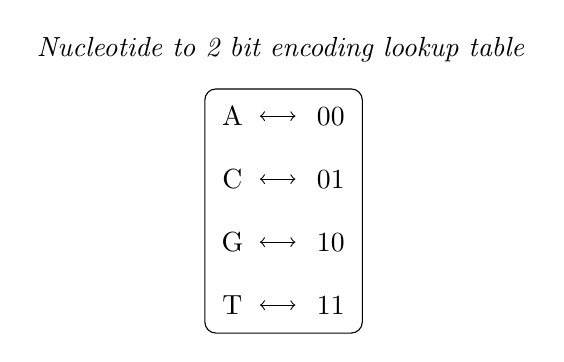
\begin{tikzpicture}
  \node at(.625,3.25)(title){\textit{Nucleotide to 2 bit encoding lookup table}};

  \node at(.65,1.195)[draw,rounded corners,minimum width=2cm,minimum height=3.1cm](lookuptable){};

  \node at(0,0)(){T};
  \node at(0,.8)(){G};
  \node at(0,1.6)(){C};
  \node at(0,2.4)(){A};

  \node at(1.25,0)(){11};
  \node at(1.25,.8)(){10};
  \node at(1.25,1.6)(){01};
  \node at(1.25,2.4)(){00};

  \draw [<->](.35,0) -- (.8,0);
  \draw [<->](.35,.8) -- (.8,.8);
  \draw [<->](.35,1.6) -- (.8,1.6);
  \draw [<->](.35,2.4) -- (.8,2.4);
\end{tikzpicture}
}

\scalebox{1}{
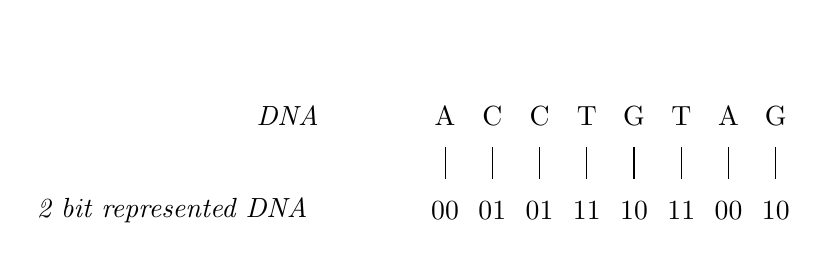
\begin{tikzpicture}
  \node at(0,1)(title){};

  \node at(-2,0)(){\textit{DNA}};
  \node at(-3.465,-1.2)(){\textit{2 bit represented DNA}};

  \node at(0,0)(){A};
  \node at(.6,0)(){C};
  \node at(1.2,0)(){C};
  \node at(1.8,0)(){T};
  \node at(2.4,0)(){G};
  \node at(3,0)(){T};
  \node at(3.6,0)(){A};
  \node at(4.2,0)(){G};

  \draw [](0,-.4) -- (0,-.8);
  \draw [](.6,-.4) -- (.6,-.8);
  \draw [](1.2,-.4) -- (1.2,-.8);
  \draw [](1.8,-.4) -- (1.8,-.8);
  \draw [](2.4,-.4) -- (2.4,-.8);
  \draw [](3,-.4) -- (3,-.8);
  \draw [](3.6,-.4) -- (3.6,-.8);
  \draw [](4.2,-.4) -- (4.2,-.8);

  \node at(0,-1.2)(){00};
  \node at(.6,-1.2)(){01};
  \node at(1.2,-1.2)(){01};
  \node at(1.8,-1.2)(){11};
  \node at(2.4,-1.2)(){10};
  \node at(3,-1.2)(){11};
  \node at(3.6,-1.2)(){00};
  \node at(4.2,-1.2)(){10};

\end{tikzpicture}
}
\caption{A lookup table showing how nucleotides can be encoded using 2 bits and a DNA nucleotide sequence represented both as plain characters as well as its 2 bit encoded representation. Recall that computers use 8 bits to represent a single nucleotide with a character, whilst the 2 bit encoding only needs 2 bits to represent a nucleotide.}
\label{background:nucleotide_binary_encoding:figures:nucleotide_binary_encoding}
\end{center}
\end{figure}


\newpage
\subsection{Biology} \label{background:biology}

\subsubsection{DNA, Chromosomes and Genomes} \label{background:biology:dna_chromosomes_and_genomes}
\textit{Deoxyribonucleic acid} (DNA) is a type of molecule that carries the genetic instructions for the development, function, and reproduction of all known living organisms.
The molecule is composed of two connected strands that wind around each other into a double helix shape.
Each strand is made up of a sugar and phosphate backbone, with each sugar carrying one out of four bases, often referred to as \textit{nucleotides}. 
The four DNA nucleotides are: \textit{cytosine}, \textit{guanine}, \textit{adenine} and \textit{thymine}, and they are typically referred to by their abbreviations C, G, A and T respectively.
Furthermore, chemical bonds form between complementary pairs of nucleotides: AT/TA and CG/GC, meaning that A and T, and C and G are complementary. 
The two strands are connected by these bonds formed between these nucleotides.
Since the sequence of nucleotides in one strand is complementary to the other, the two strands do in fact encode the same genetic information.
In other words, by having one strand, the other can be determined by reversing the strand you have and then exchanging each nucleotide by its complement.

DNA is organized into structures called \textit{chromosomes}. 
Humans have 46 chromosomes made up by two sets of 23 chromosomes where each chromosome occurs twice. One is inherited from the male parent and the other is inherited from the female parent.

The \textit{genome} of an organism usually refers to the entirety of an organism's genetic information. 

\begin{figure}[ht!]
\begin{center}
\scalebox{1}{
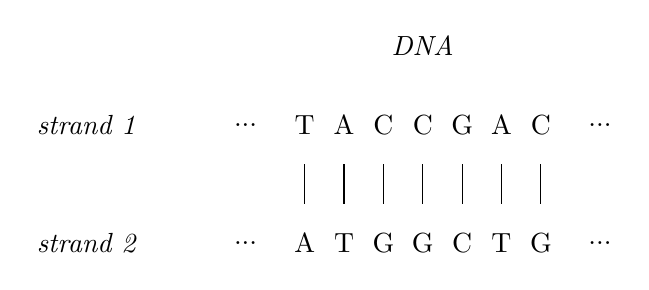
\begin{tikzpicture}
  % texts
  \node at(2.25,2.5)(title){\textit{DNA}};
  \node at(-2,0)(title){\textit{strand 2}};
  \node at(-2,1.5)(title){\textit{strand 1}};
  % lower nodes
  \node at(0,0)(n1){...};
  \node at(.75,0)(n2){A};
  \node at(1.25,0)(n3){T};
  \node at(1.75, 0)(n4){G};
  \node at(2.25,0)(n5){G};
  \node at(2.75,0)(n5){C};
  \node at(3.25,0)(n5){T};
  \node at(3.75,0)(n5){G};
  \node at(4.5,0)(n5){...};
  % upper nodes
  \node at(0,1.5)(n1){...};
  \node at(.75,1.5)(n2){T};
  \node at(1.25,1.5)(n3){A};
  \node at(1.75,1.5)(n4){C};
  \node at(2.25,1.5)(n5){C};
  \node at(2.75,1.5)(n5){G};
  \node at(3.25,1.5)(n5){A};
  \node at(3.75,1.5)(n5){C};
  \node at(4.5,1.5)(n5){...};
  % base pair bonds 
  \draw (.75,.5) -- (.75,1);
  \draw (1.25,.5) -- (1.25,1);
  \draw (1.75,.5) -- (1.75,1);
  \draw (2.25,.5) -- (2.25,1);
  \draw (2.75,.5) -- (2.75,1);
  \draw (3.25,.5) -- (3.25,1);
  \draw (3.75,.5) -- (3.75,1);
\end{tikzpicture}
}
\caption{A conceptual representation of a DNA molecule made up of two strands. The strands are composed of nucleotides forming base pairs where A (adenine) and T (thymine), and C (cytosine) and G (guanine) are complements of each other.}
\label{background:biology:dna_and_chromosomes:figures:dna_strands}
\end{center}
\end{figure}

Studying organisms' DNA is important for a variety of reasons.
It is particularly important to understand genetic diseases and how to best treat them.

...

\subsubsection{High-Throughput DNA Sequencing} \label{background:biology:high_throughput_dna_sequencing}
\textit{High-throughput sequencing} (HTS), also known as \textit{next-generation sequencing} (NGS), refers to an assortment of recently developed technologies that parallelize the sequencing of DNA fragments to provide unprecedented amounts of genomic sequence data in short amounts of time.
While several such technologies with varying details exist today, they commonly follow a general paradigm. 
%This paradigm consists of performing a template preparation, clonal amplification where they clone pieces of DNA in order to sequence the clones in parallel, and finally cyclical rounds of massively parallel sequencing \cite{hts}.
This paradigm consists of performing a template preparation, clonal amplification where pieces of DNA are cloned in order to sequence the clones in parallel, and finally, cyclical rounds of massively parallel sequencing \cite{hts}.
The resulting DNA sequences produced by HTS technologies are usually referred to simply as (DNA) \textit{reads}.
Such reads are commonly stored as plain text in FASTA or FASTQ files, which can later be used for different kinds of analysis such as genotyping.
Depending on which HTS technology is used, one can expect read lengths ranging from as low as 150 bases using \textit{Illumina} technologies, referred to as \textit{short reads} \cite{illumina_read_length}, all the way up to 15-20 thousand bases using \textit{Pacific Biosciences} (PacBio) technologies, referred to as \textit{long reads} \cite{hts2}.
There are three important factors to consider when determining which HTS technology to use for a given purpose: 1) the read lengths produced, 2) the average probability for each base being erroneous, usually referred to as the error rate, and 3) the cost of sequencing given the technology, which can potentially limit how much data one may be able to produce.

\begin{figure}[H]
\begin{center}
\small{example.fa}
\end{center}
\begin{lstlisting}[style=vcf]
>read 0
ACGTATGCGGCGGGGCGCGATTATTCGTTGCGTATGC
>read 1
ACACGTCGTGCGTAGCGTGTCAGTCACAGTAAACAAA
>read 2
CGTTGCCATCAACGGCTGTGCACGATTGGGGGCGCGC
...
\end{lstlisting}
\caption{
  An illustration of how sequenced DNA reads are stored as plain text in a FASTA (.fa) file.
  Before each read, a header file beginning with the character ">" may provide information about the read.
}
\label{background:biology:high_throughput_dna_sequencing:figures:fasta}
\end{figure}

When performing DNA sequencing, we have no knowledge of where a read originates from in the original genome.
This issue, in addition to the fact that some bases are erroneously sequenced, introduces uncertainties when trying to predict features about an individual's genome based on the sequenced reads.
Many techniques rely on \textit{aligning} (or \textit{mapping}) sequenced reads to a reference genome sequence in order to better predict where in the genome the read originates from.
To gain better confidence and local support along these alignments, it is common to sequence an individual's genome at higher coverages, so that aligned reads may overlap and correspondance can be asserted.
The term sequencing \textit{coverage} is used as an indication of how many times each nucleotide in a genome has been sequenced on average.
E.g. 15x coverage means that every nucleotide in the genome has been sequenced, on average, 15 times.

\subsubsection{Variants and Variant Calling} \label{background:biology:variants_and_variant_calling}
When examining the genome of several individuals within the same species, one will find locations along the genome where the nucleotides differ for the different individuals.
These distinct nucleotide manifestations are commonly referred to as \textit{variants}.
The term \textit{variant calling} is used to refer to the process of determining which variants an individual has.
In other words, given a reference genome sequence, where and how does the genome sequence of the individual of interest differ from the reference sequence.
This process can abstractly be described in three steps: 
1) sequence the genome of interest to get DNA reads (described in section \ref{background:biology:high_throughput_dna_sequencing}), 
2) align the reads to the reference genome by finding where along the reference genome sequence each read fits best, usually using a heuristic determining which location the read actually originates from, and 
3) examine the alignments and note where the reads differ from the reference sequence, determining the variants present in the sequenced genome \cite{variant_calling}.



\subsubsection{Genotypes and Genotyping} \label{background:biology:genotype_and_genotyping}
Much like variant, the term \textit{genotype} is used slightly ambiguously in the world of bioinformatics. 
The term genotype may be used to refer to an individual's total genetic makeup.
It may also refer to the variants an individual carries in its chromosomes at a particular location along the genome.
Throughout this thesis, we assume the latter definition.
For humans, who have two copies of each chromosome, we may have the same or two different variations present at a particular location in the genome, making up the genotype.

\textit{Genotyping} an individual refers to the process of determining which genotypes an individual carries. 
For humans, this would entail determining the set of variants present at each variant site.
In most genotyping software tools today, genotypes are given in a format that specifies whether a particular variant is present in none, one or both of a human's chromosomes.
For instance, given a reference genome sequence where a variant site is known to could manifest an A at a particular allele where the reference sequence contains a G, a human individual's genotype for this variant could either be referred to as $0/0$, meaning that the variant allele A is present in neither of the chromosomes, $0/1$, meaning that it is present in one of the chromosomes, or $1/1$, meaning that it is present in both chromosomes.

\definecolor{variantcolor}{RGB}{235,235,235}

\begin{figure}[H]
\begin{center}
\scalebox{0.85}{
\begin{tikzpicture}
  % Variants
  \node at(2.25,2)(title){\textit{Variants}};
  \node at(2.25,0)[rounded corners,minimum width=0.5cm,minimum height=2.75cm, fill=variantcolor](variant){};
  % Sequence (left)
  \node at(0.75,0)(n2){\large A};
  \node at(1.25,0)(n3){\large T};
  \node at(1.75,0)(n4){\large G};
  \node at(2.25,1)(n5){\large A};
  \node at(2.25,0)(n5){\large G};
  \node at(2.25,-1)(n5){\large C};
  \node at(2.75,0)(n5){\large C};
  \node at(3.25,0)(n5){\large T};
  % Arrow
  %\draw [-stealth](4,0) -- (5,0);
  %\draw [thick,->](4,0) -- (5,0);
  \draw [double distance=1pt,->](4,0) -- (5,0);
  % Genotype
  \node at(7.5,2.5)(title){\textit{Genotype}};
  \node at(9,0.25)[rectangle,rounded corners,draw,minimum width=7cm,minimum height=3.25cm](genotype){};
  % Alleles 
  \node at(7.5,1.5)(title){\textit{Alleles}};
  % Chromosomes
  \node at(10.5,0.5)(title){\textit{Chromosome}$_1$};
  \node at(10.5,-0.5)(title){\textit{Chromosome}$_2$};
  \node at(7.5,-.015)[rounded corners,minimum width=0.5cm,minimum height=1.75cm, fill=variantcolor](variant){};
  % Chromosome 1 sequence
  \node at(6,0.5)(n2){\large A};
  \node at(6.5,0.5)(n3){\large T};
  \node at(7,0.5)(n4){\large G};
  \node at(7.5,0.5)(n5){\large A};
  \node at(8,0.5)(n5){\large C};
  \node at(8.5,0.5)(n5){\large T};
  % Chromosome 2 sequence
  \node at(6,-0.5)(n2){\large A};
  \node at(6.5,-0.5)(n3){\large T};
  \node at(7,-0.5)(n4){\large G};
  \node at(7.5,-0.5)(n5){\large G};
  \node at(8,-0.5)(n5){\large C};
  \node at(8.5,-0.5)(n5){\large T};
  % Reference and the individual's chromosomes
  \node at(2.25,-2.5)(ref){\textit{Reference sequence}};
  \node at(9,-2.5)(ind){\textit{Individual's chromosome sequences}};
\end{tikzpicture}
}
\caption{
  In humans, who carry two copies of every chromosome, a genotype constitutes a set of two alleles or variants - one in each chromosome at the variant site. 
  Along the reference sequence on the left, several possible variants may be known to occur at a specific site. 
  After examining the sequence of an individual, we try to determine the individual's genotype by scoring which variants are present in each chromosome at the location of interest.
  In this illustration, the individual's genotype may be described as two scores: $0/1$ for the SNP variant where the G is replaced by an A in chromosome$_1$, and $0/1$ for the G remaining the same as in the reference in chromosome$_2$.
}
\label{figure:variant_and_genotype}
\end{center}
\end{figure}

Today, the most established ways to genotype individuals are based on \textit{alignment-based} methods.
Such methods rely on aligning sequenced DNA reads to a reference genome and performing variant calling before calling genotypes by assessing which genotypes are most probable based on locally supported variants \cite{gatk}.
However, given the vast amount of reads provided by high-throughput sequencing technologies today, aligning each read to a $3*10^9$ long reference sequence is very compute, memory and time consuming.
As a result, a set of new prominent methods have emerged in recent years to help alleviate these issues.
\textit{Alignment-free} genotyping methods, where the alignment of reads and variant calling step are skipped altogether, have yielded promising results and significant speedup compared to their alignment-based counterparts.
In such methods, small parts of the sequenced reads called \textit{k}mers are analyzed, and statistical models are used to compute genotype-probabilities supported by the results from the \textit{k}mer analysis and previous knowledge of variants and genotypes that have been accumulated over years of research \cite{kage,malva,1000_genomes_project}.
One such alignment-free genotyper, KAGE, has recently shown that it can genotype a human individual more than 10 times faster than any other known genotyper tool, while still providing competitive accuracy scores for its genotype calls \cite{kage}.



\newpage
\section{Methods} \label{methods}

In this section we describe how GPU acceleration support was provided for the KAGE genotyping pipeline, resulting in GKAGE - a version of KAGE where parts of the pipeline is GPU accelerated.
We will give an account of how we determined which parts to focus on GPU accelerating, and describe a testing strategy that we deployed that allowed us to GPU accelerate existing NumPy code directly in Python to see whether significant runtime speedup was plausible.
Then, we will describe how we implemented the solutions that were introduced into KAGE, resulting in GKAGE.


\subsection{GPU Support Directly in Python} \label{methods:gpu_support_directly_in_python}
...

\subsection{Custom CUDA Implementations} \label{methods:custom_cuda_implementations}
...

\subsection{Finding Bottleneck Components} \label{methods:finding_bottleneck_components}
...


\subsection{Implementation Details}

\input{sections/methods/implementation_details/cuda_hashtable.tex}


%\input{sections/methods/cuda_hashtable.tex}

\newpage
\section{Results} \label{results}

In the following section we will present the final GPU accelerated version of KAGE, GKAGE, and benchmark it against KAGE on two different computer systems to evaluate the final speedup achieved by GPU acceleration.


\subsection{\textit{K}mer parsing from raw reads}
Section (methods:cupy...) describes how GPU support was implemented for parts of BioNumPy \cite{bionumpy} in order to allow for GPU acceleration when when parsing \textit{k}mers from raw reads in FASTA files.
In short: BioNumPy reads and parses chunks of \textit{k}mers from FASTA files by 
1) reading a chunk of raw bytes from the FASTA file, 
2) converting each DNA nucleotide found in the raw read data into 2-bit encoded representations [\ref{background:nucleotide_binary_encoding}], 
and 3) parsing all valid \textit{k}mers of the desired size from the 2-bit encoded reads data.

After copying the raw bytes that were read into memory from the FASTA file directly to the GPU memory, steps 2) and 3) could be performed significantly faster on the GPU for large enough chunk sizes, given the high throughput of the GPU.

...

\subsection{\textit{K}mer counting}
...

\subsection{GKAGE vs KAGE} \label{results:gkage_vs_kage}
...



\newpage
\section{Discussions} \label{discussions}

\subsection{Implementing Our Own \textit{k}mer Counting Tool} \label{discussion:implementing_our_own_kmer_counting_tool}
In section \ref{results:benchmarking:runtimes} we showed that Gerbil's \cite{gerbil} runtime was greater than that of GKAGE despite Gerbil only performing \textit{k}mer counting and GKAGE performing the full genotyping pipeline.
The reason for why we decided to implement our own tool for \textit{k}mer counting on the GPU and why it seemingly performs so much better than Gerbil is because the problems solved by Gerbil and GKAGE's \textit{k}mer counting tool are inherently different.
Recall from section \ref{background:kmers_and_kmer_counting}, we defined \textit{full k}mer counting as the problem of counting the occurrence of every valid \textit{k}mer in a set of reads, and \textit{partial k}mer counting as the problem of only counting the occurrences of \textit{k}mers present in a predefined set of \textit{k}mers in a set of reads.
Gerbil, unlike the \textit{k}mer counting tool we implemented for GKAGE, solves the \textit{full k}mer counting problem - a significantly more processing and memory demanding task compared to \textit{partial k}mer counting.
While Gerbil could have been used in GKAGE for the \textit{k}mer counting portion, we would not only be counting the occurrences of superfluous \textit{k}mers, we would additionally be required to parse Gerbil's output for the wanted \textit{k}mer counts.
It was for this reason that we decided on implementing a new \textit{k}mer counting tool targeted for our particular purpose.

\subsection{Advantages and Drawbacks of Methods} \label{discussion:advantages_and_drawbacks_of_methods}
In section \ref{methods} we explored three different methods for GPU accelerating existing Python code.
Each of the methods we explored has a unique set of advantages and drawbacks.
The discipline of designing and implementing GPU programs is quite distinct from the more mainstream discipline of implementing programs meant to run serially on the CPU.
Becoming an expert GPU programmer can in many instances take years with all the technologies and tools available today.
Thus, an interesting dimension when assessing the advantages and drawbacks of the GPU acceleration methods we have explored is how seamless it is to implement the solution, particularly for someone with little or no experience in GPU programming.
%Other metrics we will discuss include how seamless the integration of a solution into Python is, how quickly a solution can be implemented compared to the alternative methods, among other per-method details.
We will additionally consider how seamless integration into Python is, and of course, the potential for performance.

\subsubsection{Using CuPy as a NumPy Drop-in Replacement} \label{discussion:using_cupy_as_a_numpy_drop_in_replacement}
The first GPU acceleration method we explored in section \ref{methods:preliminary_testing}, was to use CuPy, a GPU accelerated array library with an interface designed to closely follow NumPy, as a drop-in replacement for NumPy. 

\paragraph{Advantages}
This method is ideal in cases where an already existing Python solution based on NumPy exists.
Depending on the complexity of the program architecture, replacing the NumPy module with CuPy can yield seamless and immediate GPU acceleration without the need to implement any GPU functionality, understand the GPU hardware or leave the Python ecosystem.
This technique is in such instances, by a large margin, the fastest way of implementing GPU acceleration.
In cases where no existing solution exists to transform, CuPy is still an adequate tool for "quick and dirty" testing with seamless GPU acceleration directly in Python.
Additionally, this method does not require deep knowledge or understanding of the GPU hardware and architecture, as the routines and functions are implemented by the CuPy developers.
That being said, some knowledge about GPUs may still be helpful, as it can guide decision making about what type of NumPy code may best be suited for GPU acceleration and how the data flow may be best optimized.

\paragraph{Drawbacks}
While an advantage of CuPy is that it allows for seamless "quick and dirty" testing directly in Python, this conversely also introduces a drawback of this method.
Many solutions implemented using NumPy are designed for fast processing on the CPU.
While such solutions may seem like good candidates for GPU acceleration, this match is not guaranteed.
Additionally, because NumPy and CuPy are Python libraries, they suffer from many unnecessary data allocations and copies when nested Python expressions with arrays are computed.
An example highlighting this issue is the log of the probability mass function (LOGPMF) described in section \ref{methods:gpu_accelerating_genotyping}.
As the nested LOGPMF expression is computed using CuPy arrays, Python's evaluation rules dictate that the expression must be evaluated one operation at a time.
Thus, a simple expression may allocate and produce many temporary arrays, although only a single output array remains when the expression is fully computed.
These allocations and copies result in a significant spike in global memory requests and memory usage on the GPU, and can be circumvented when implementing custom kernels using either CuPy's JIT compiled kernel support or CUDA in C++.

\subsubsection{Custom C++ Implementations Using CUDA}
The second GPU acceleration method we explored in section \ref{methods:gpu_accelerating_kmer_counting}, was to implement our own solution directly in C++ using the CUDA framework.
We then used pybind11 to create Python bindings for our C++ functionality to gain access directly inside Python.

\paragraph{Advantages}
The clearest advantage of this method is the granular control over the hardware achieved when implementing the solution directly in Nvidia's programming platform: CUDA.
This provides the possibility of closely tailoring the implementation to the problem and using all of CUDA's technologies to optimize and gain the best performance possible.
Additionally, since such an implementation would be created using C++, this allows access to C++ features that are otherwise out of reach in Python, such as thread parallelization.

\paragraph{Drawbacks}
For this method too, its main advantage also yields its greatest drawback.
The CUDA programming platform is vast and provides support that can be extremely useful to solve certain problems effectively, but that also requires deep knowledge and understanding of the GPU hardware- and programming model.
Additionally, since CUDA features are used in C++, the programmer would need to be, at the very least, comfortable with writing software in C++.
Integration to Python also becomes significantly more difficult, as solution are implemented in C++.
Python bindings, using tools such as ctypes or pybind11, are necessary to integrate solutions into the Python ecosystem.
This, in addition to the fact that C++ is a significantly more verbose language than Python, results in production time being vastly greater for solutions implemented using this method, even for an experienced CUDA programmer.

\subsubsection{Custom JIT-Compiled Kernels in Python}
The third and final GPU acceleration method we explored in section \ref{methods:gpu_accelerating_kmer_counting_jit}, was to implement our solution using CuPy's support for JIT (just-in-time) compiled custom kernels.
CuPy, directly in Python through its module interface, provides access to certain CUDA functionality as well as support for creating kernels directly in Python code that are then compiled when the program first encounters them.

\paragraph{Advantages}
This method has many of the same advantages as the method discussed in \ref{discussion:using_cupy_as_a_numpy_drop_in_replacement}, and can be viewed as an extension of the CuPy drop-in for NumPy method.
What it brings in addition to being a drop-in replacement for NumPy is its JIT compiled custom kernel support and, although limited, CUDA functionality support.
This allows for simple array-programming similar to NumPy where it is suitable, and more detailed usage with custom kernels and some other CUDA functionality in cases where the straight-forward array-interface does not suffice.
In section \ref{methods:gpu_accelerating_kmer_counting_jit}, we showed that we could fully re-implement our CUDA hash table directly in Python using CuPy's custom kernel support.
This was all achieved while never leaving Python, meaning a programmer does not need to know C++ in order to implement custom kernels this way.
More additional functionality not used in our implementation of GKAGE is also supported through CuPy, such as CUDA streams cooperative groups and more \cite{cupy}.

\paragraph{Drawbacks}
While it is helpful to be able to implement custom kernels directly in Python code, it is uncertain how much simplicity this in effect introduces.
The kernels implemented using CuPy's custom kernel support still need to adhere to the same programming model as CUDA kernels implemented in C++.
A programmer with little or no knowledge of how the GPU hardware and programming model works will not with ease be able to implement effective kernels this way.
Therefore, we would argue that this advantage does not do much more than alleviate the need to delve into C++ and set up proper compiling and Python bindings.

\subsection{Drawbacks of Graphical Processing Units}
While GPUs can provide excellent acceleration for many problems in scientific computing, they do come with some notable caveats.

The reason why GPUs are powerful when it comes to accelerating certain parallel programs, is because they are designed for such problems.
GPUs are highly specialized compute accelerators that perform poorly when applied to any problem that does not fit its compute architecture.
Additionally, today's GPUs are expensive and less accessible than traditional CPUs.
Because of the CPU's flexibility in regards to the problems it can solve, CPUs exist in most - if not all - existing computers today.
GPUs, however, are less common, partly because of cost.

Furthermore, GPU programming is its own discipline, as the programming models and paradigms used when developing GPU programs are quite different from the typical sequential programs written for the CPU.
This leads to a higher bar for entry when it comes to developing effective GPU programs for difficult problems, as fewer expert programmers have the knowledge and training to implement such solutions.


\subsection{Further Work}
While GKAGE demonstrates that alignment-free genotyping can be sped up through GPU acceleration, we believe that the current GKAGE runtimes can still be significantly improved.
We will here identify some possible avenues where the current implementation can be altered or improved in order to better use the hardware and technology available to gain more speedup.

\subsubsection{Better GPU Hash Table}
While the GPU hash table used in GKAGE for \textit{k}mer counting is plenty effective for our purpose of demonstrating the effectiveness of GPU acceleration in alignment-free genotyping, alternative hash tables exist that, with correct integration, should perform better.
Since optimizing GPU hash tables can be considered a discipline in and of itself, and beyond the scope of this thesis, our GPU hash table implements a naive solution for collision handling and probing.
An interesting avenue would be to integrate a version of a bucketed static cuckoo hash table from Awad et al., (2023) \cite{bght} to evaluate how a state-of-the-art GPU accelerated hash table would perform compared to our own implementation.
%Although faster, we doubt the effect would be dramatic in our case.

\subsubsection{Parallelization of \textit{k}mer Chunk Preparation}
Recall that in the \textit{k}mer counting step in KAGE, the input FASTA file is read in chunks.
Each chunk of data is then 2-bit encoded and all valid \textit{k}mers are hashed from the 2-bit encoded data chunk.
Finally, the chunk of hashed \textit{k}mers are counted.
In GKAGE, the 2-bit encoding, \textit{k}mer hashing and \textit{k}mer counting are performed on the GPU.
Thus, the chunk of data read from the FASTA file is copied to the GPU's memory before processing begins.
Currently, GKAGE performs all of these processes sequentially.

\vspace{.5em}
\begin{figure}[H]
\begin{center}
\scalebox{.92}{
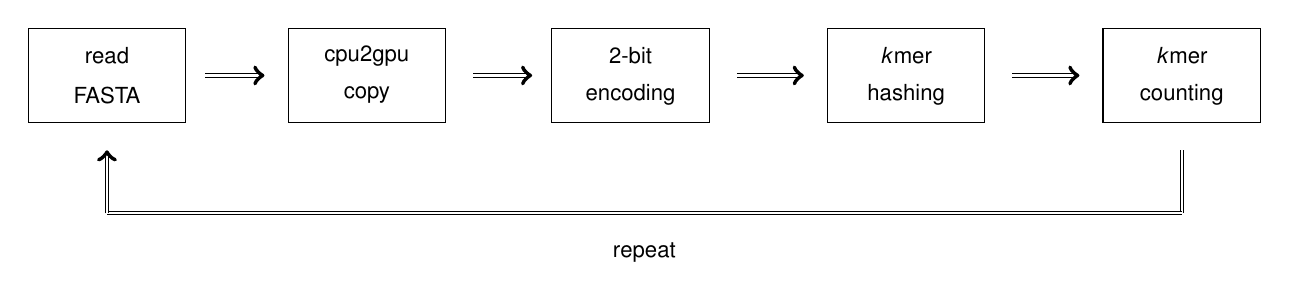
\begin{tikzpicture}
  % read fasta
  \node at(0,0)[draw,minimum width=2cm,minimum height=1.2cm](start){};
  \node at(0,.25)[]{\fontfamily{phv}\selectfont\smaller{read}};
  \node at(0,-.25)[]{\fontfamily{phv}\selectfont\smaller{FASTA}};
  \draw [double distance=.75pt,->](1.25,0) -- (2,0);
  % cpu2gpu copy
  \node at(3.3,0)[draw,minimum width=2cm,minimum height=1.2cm]{};
  \node at(3.3,.25)[]{\fontfamily{phv}\selectfont\smaller{cpu2gpu}};
  \node at(3.3,-.25)[]{\fontfamily{phv}\selectfont\smaller{copy}};
  \draw [double distance=.75pt,->](4.65,0) -- (5.4,0);
  % 2-bit encoding
  \node at(6.65,0)[draw,minimum width=2cm,minimum height=1.2cm]{};
  \node at(6.65,.25)[]{\fontfamily{phv}\selectfont\smaller{2-bit}};
  \node at(6.65,-.25)[]{\fontfamily{phv}\selectfont\smaller{encoding}};
  \draw [double distance=.75pt,->](8,0) -- (8.85,0);
  % kmer hashing
  \node at(10.15,0)[draw,minimum width=2cm,minimum height=1.2cm]{};
  \node at(10.15,.25)[]{\fontfamily{phv}\selectfont\smaller{\textit{k}mer}};
  \node at(10.15,-.25)[]{\fontfamily{phv}\selectfont\smaller{hashing}};
  \draw [double distance=.75pt,->](11.50,0) -- (12.35,0);
  % kmer counting
  \node at(13.65,0)[draw,minimum width=2cm,minimum height=1.2cm](end){};
  \node at(13.65,.25)[]{\fontfamily{phv}\selectfont\smaller{\textit{k}mer}};
  \node at(13.65,-.25)[]{\fontfamily{phv}\selectfont\smaller{counting}};
  % arrows
  \draw [double distance=.75pt](13.65,-.95) -- (13.65,-1.75);
  \draw [double distance=.75pt](13.65,-1.75) -- (0,-1.75);
  \draw [double distance=.75pt,->](0,-1.75) -- (0,-.95);
  \node at(6.825,-2.25)[]{\fontfamily{phv}\selectfont\smaller{repeat}};
\end{tikzpicture}
}
\caption{
  GKAGE's current \textit{k}mer counting pipeline performs several steps in a sequential fashion.
  While these steps are performed on many \textit{k}mers in parallel at once, each chunk (containing many \textit{k}mers) is processed sequentially. 
}
\label{discussion:parallelization_of_kmer_chunk_preparation:figures:pipeline}
\end{center}
\end{figure}

By utilizing CUDA streams we can parallelize the copying of data to the GPU and the processing of the previous chunk, creating a new and more efficient pipeline.

\begin{figure}[H]
\begin{center}
\scalebox{.9}{
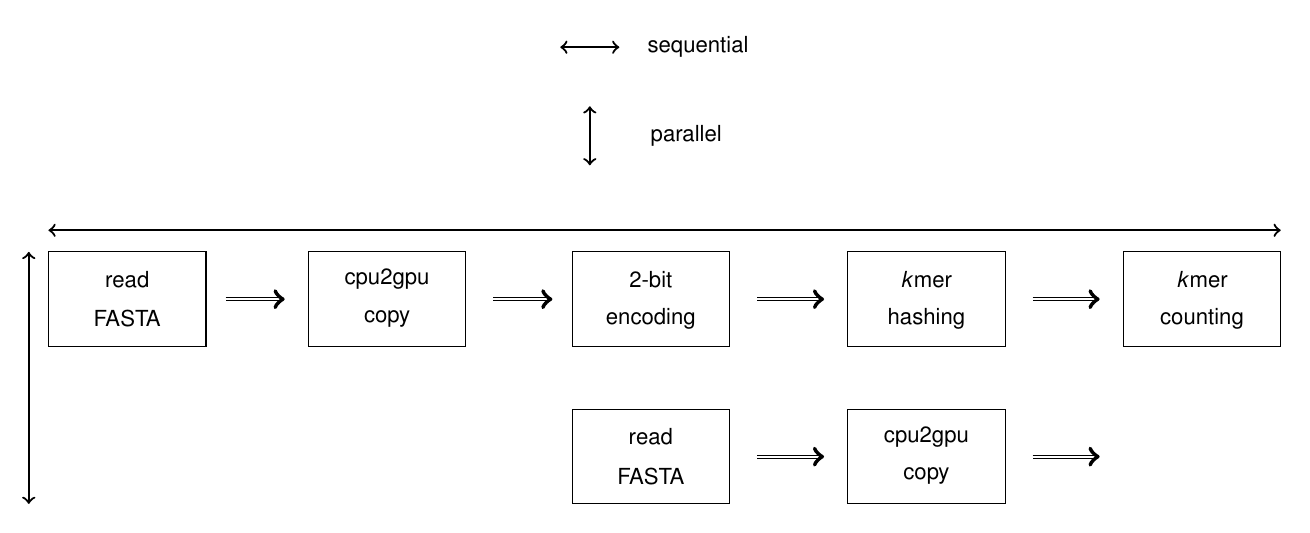
\begin{tikzpicture}
  % hints
  \draw [thick,<->](5.875,2.45) -- (5.875,1.7);
  \node at(7.1,2.075)[]{\fontfamily{phv}\selectfont\smaller{parallel}};
  \draw [thick,<->](5.5,3.2) -- (6.25,3.2);
  \node at(7.25,3.2)[]{\fontfamily{phv}\selectfont\smaller{sequential}};
  % large hints
  \draw [thick,<->](-1.25,.6) -- (-1.25,-2.6);
  \draw [thick,<->](-1,.875) -- (14.65,.875);
  % read fasta
  \node at(0,0)[draw,minimum width=2cm,minimum height=1.2cm](start){};
  \node at(0,.25)[]{\fontfamily{phv}\selectfont\smaller{read}};
  \node at(0,-.25)[]{\fontfamily{phv}\selectfont\smaller{FASTA}};
  \draw [double distance=.75pt,->](1.25,0) -- (2,0);
  % cpu2gpu copy
  \node at(3.3,0)[draw,minimum width=2cm,minimum height=1.2cm]{};
  \node at(3.3,.25)[]{\fontfamily{phv}\selectfont\smaller{cpu2gpu}};
  \node at(3.3,-.25)[]{\fontfamily{phv}\selectfont\smaller{copy}};
  \draw [double distance=.75pt,->](4.65,0) -- (5.4,0);
  % 2-bit encoding
  \node at(6.65,0)[draw,minimum width=2cm,minimum height=1.2cm]{};
  \node at(6.65,.25)[]{\fontfamily{phv}\selectfont\smaller{2-bit}};
  \node at(6.65,-.25)[]{\fontfamily{phv}\selectfont\smaller{encoding}};
  \draw [double distance=.75pt,->](8,0) -- (8.85,0);
  % kmer hashing
  \node at(10.15,0)[draw,minimum width=2cm,minimum height=1.2cm]{};
  \node at(10.15,.25)[]{\fontfamily{phv}\selectfont\smaller{\textit{k}mer}};
  \node at(10.15,-.25)[]{\fontfamily{phv}\selectfont\smaller{hashing}};
  \draw [double distance=.75pt,->](11.5,0) -- (12.35,0);
  % kmer counting
  \node at(13.65,0)[draw,minimum width=2cm,minimum height=1.2cm](end){};
  \node at(13.65,.25)[]{\fontfamily{phv}\selectfont\smaller{\textit{k}mer}};
  \node at(13.65,-.25)[]{\fontfamily{phv}\selectfont\smaller{counting}};
  % read fasta 2
  \node at(6.65,-2)[draw,minimum width=2cm,minimum height=1.2cm](start){};
  \node at(6.65,-1.75)[]{\fontfamily{phv}\selectfont\smaller{read}};
  \node at(6.65,-2.25)[]{\fontfamily{phv}\selectfont\smaller{FASTA}};
  \draw [double distance=.75pt,->](8,-2) -- (8.85,-2);
  % cpu2gpu copy 2
  \node at(10.15,-2)[draw,minimum width=2cm,minimum height=1.2cm]{};
  \node at(10.15,-1.75)[]{\fontfamily{phv}\selectfont\smaller{cpu2gpu}};
  \node at(10.15,-2.25)[]{\fontfamily{phv}\selectfont\smaller{copy}};
  \draw [double distance=.75pt,->](11.5,-2) -- (12.35,-2);
\end{tikzpicture}
}
\caption{
  An illustration of a more optimal \textit{k}mer counting pipeline.
  By utilizing CUDA's streams, we can parallelize copying of data to the GPU and actual GPU processing.
}
\label{discussion:parallelization_of_kmer_chunk_preparation:figures:parallel_pipeline}
\end{center}
\end{figure}



\newpage
\section{Conclusion} \label{conclusion}
In section \ref{introduction:thesis_goals}, we stated that one of the two goals of this thesis was to explore whether alignment-free genotyping could be sped up in any significant way by using the GPU.
To investigate this, we attempted to GPU accelerate an existing genotyper, KAGE, which recently showed that it was an order of magnitude faster than any other known genotyper \cite{kage}.
As a result of GPU accelerating components of KAGE, we presented GKAGE (GPU KAGE), a new GPU accelerated version of KAGE.
GKAGE achieves up to 5X speedup compared to KAGE on a high-end compute server, and more than 10X speedup on commercial hardware, all while using very little GPU memory - a scarce resource.
We believe that GKAGE is a useful contribution to the world of bioinformatics, considering the rate of which whole-genome sequencing is becoming more accessible and tools to analyze the generated sequence data is becoming increasingly necessary.

The second goal we presented in section \ref{introduction:thesis_goals}, was to investigate and experiment with different ways of GPU accelerating existing Python code that relies on array-programming libraries such as NumPy \cite{numpy}, and to reveal the advantages and drawbacks of such methods.
We achieved this by GPU accelerating different components of KAGE using a suite of different methods.
For each method, we discussed its advantages and drawbacks, where dimensions such as ease-of-use, seamless integration and performance were central.
We see the insights revealed by exploring these methods as showing that GPU acceleration is a feasible avenue to unlock performance enhancements in existing tools, particularly tools relying on large array-computations.
%As large array-computations are commonplace in computational biology, and as GPU acceleration libraries such as CuPy \cite{cupy} are making GPU acceleration more accessible even to programmers without much knowledge about GPUs, we believe that there could be an avalanche of existing methods and tools that could benefit from integrating such acceleration.
Large array-computations are commonplace in computational biology.
Additionally, Python GPU acceleration libraries such as CuPy \cite{cupy} are making GPU acceleration more accessible, even to programmers with limited knowledge of the GPU's programming model and hardware.
Given these factors, we believe that there could be an avalanche of existing methods and tools that could greatly benefit from integration such acceleration.


% bibliography
\newpage
\printbibliography

\end{document}
